\newcommand{\projectName}{Az EGTIB}

\section{\projectName{} bemutatása}

\projectName{} projekt célja egy olyan felhasználóbarát felület, mely lehetőséget teremt a daganatos sejtek játékelméleti modellezésére és szimulációjára, valamint a szimulációs eredmények megjelenítésére. Ezért született meg, a mai trendeket figyelembe véve, egy kliens-szerver architektúrán alapuló webalkalmazás, mely részben a\cite{archetti2016cooperation}-ben megjelent modellt implementálja, és ahhoz új funkcionalitásokat is hozzáad.

\begin{figure}[ht!]
	\centering
	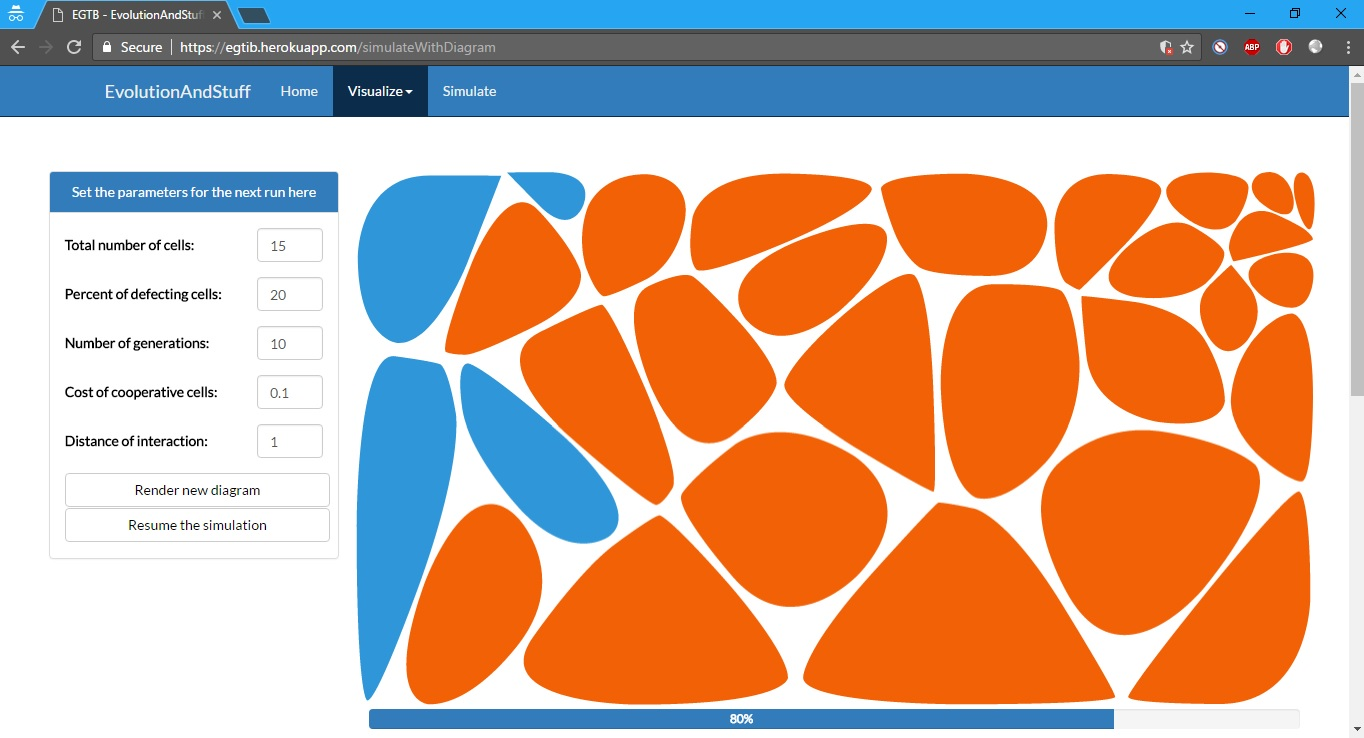
\includegraphics[width=90mm]{images/EGTIB.jpg}
	\caption{Pillanatkép az alkalmazásról \label{fig:SimulateWithDiagram}}
\end{figure}

\subsection{Funkcionalitások}

Megfelelve a követelményeknek melyeket a "megrendelő" állított fel, a felhasználónak lehetősége van bizonyos paramétereket megválasztani még a szimulálási fázis előtt:
\begin{itemize}[noitemsep]
	\item kezdeti populáció mérete
	\item defektálók aránya 
	\item generáció szám (szimuláció hossza)
	\item kooperáló sejtek termelési költsége 
	\item diffúziós távolság mérete
	\item akarja-e a felhasználó, hogy a sejtek osztódásra legyenek képesek
\end{itemize}
Ezen paramétereket felhasználva kigenerálható egy voronoi diagram mely a sejteket ábrázolja. A simulate gombot megnyomva ez az adatcsomag eljut a szerverhez amely elvégzi az erőforrás igényes számításokat melynek eredményét visszaküldi a kliensnek, ami majd azt megjeleníti.
Az alkalmazásunkat felhasználási szempontból két fő komponensre oszthatjuk:

\paragraph{Vizualizáció}- képes szimulálni kevés sejtből (max. 500) álló populációkat és ezeket generációnként meg is tudja jeleníteni. A megjelenítés interaktív, ami azt jelenti, hogy bármikor meg lehet állítani, folytatni vagy akár tekergetni mint egy filmet. Továbbá mindehhez tartozik egy grafikon is, mely a populációnak változását ábrázolja generációnként.

\paragraph{Szimuláció}- alkalmas nagyobb (max. 2000) populációval dolgozni, viszont ezek megjelenítése már túl sok időt venne igénybe, így csak a fentebb említett grafikon segítségével ábrázolja azt, hogy mi is történik a sejtek között. Előnye a vizualizációs részhez képest elsősorban az, hogy sokkal nagyobb populációval tud dolgozni, de a paraméterlista is változatosabb (a szimuláció során használt függvények viselkedésébe is bele tud szólni a felhasználó) és hatalmas kényelmi faktornak számít az, hogy több, különböző paraméterezésű szimulációt is képes egy gombnyomással lekérni.

\subsection{Felhasznált technológiák}

A szoftver egy szerverből és egy kliensből áll, melyek közötti kommunikáció a már jól megszokott HTTP mellett, websocketen keresztül is folyik. Az utóbbira azért van szükség, mert gyorsítja az adatok áramlását, és alkalmas nagyobb mennyiségű adat átvitelére, mely a szimuláció során keletkezik. 

Kliens oldali technológiák közé sorolandó a Bootstrap\cite{soft:bootstrap}, mely segítségével nem csak desktopon de mobil platformon is elegáns az oldal kinézete, valamint az AngularJS\cite{soft:angular}, ami biztosítja az oldal dinamikusságát. A Paper.js\cite{soft:paper} a rajzok megjelenítéséért felelős, és ennek egy segédkönyvtára\cite{soft:voronoiModule} pedig kifejezetten a voronoi diagram ábrázolásáért, úgy vizuálisan mint adatszerkezeti szinten is. A grafikonok kirajzolását kezdetben a Highchartsra\cite{soft:highcharts} míg a későbbiekben a könnyebben használható Plotly.js-re\cite{soft:plotly} bíztuk.

A szerverünk NodeJS\cite{soft:node} alapú, az Express\cite{soft:express} keretrendszert használja fel. Itt folyik az erőforrás igényes számítások nagy része, így itt is jelen van a Paper.js voronoi modulja\cite{soft:voronoiModule}.

Mindezt összefogva és belerakva egy Dockerbe\cite{soft:docker}, már mehet is egy felhőbe, a mi esetünkben ez a Heroku (https://egtib.herokuapp.com/). A fejlesztési és tesztelési folyamatot amennyire csak lehetett megpróbáltuk automatizálni, így a Travis CI\cite{soft:travis} az, ami a projektünket teszteli és amennyiben szükséges kitelepíti a legújabb verziót a felhőbe.

Az alkalmazásunk minőségét unit és E2E tesztekkel próbáltuk meg biztosítani, ezekhez a Mocha\cite{soft:mocha} és TestCafe\cite{soft:testcafe} keretrendszereket használtuk.

\begin{figure}[ht!]
	\centering
	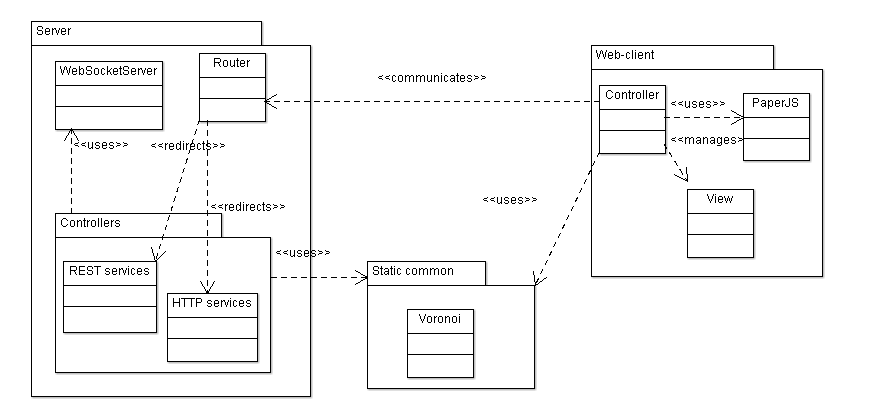
\includegraphics[width=\linewidth]{images/Architecture}
	\caption{A projekt architektúrája\label{fig:Architecture}}
\end{figure}
